% @Author: Athul Vijayan
% @Date:   2014-05-09 13:56:20
% @Last Modified by:   Athul
% @Last Modified time: 2016-02-25 11:44:16

\documentclass[11pt,paper=a4,answers]{exam}
\usepackage{graphicx,lastpage}
\usepackage{subcaption}
\usepackage[table]{xcolor}

\usepackage{multirow}
\usepackage{upgreek}
% \usepackage{float}
\usepackage{placeins}
\usepackage[bookmarks]{hyperref}
\usepackage{censor}
\usepackage{amsmath}
\usepackage{amssymb, amsthm}
\newcommand{\argmax}{\operatornamewithlimits{argmax}}
\usepackage{bm}
\usepackage{caption}
\usepackage{morefloats}
\usepackage{enumerate}


\newcommand{\cb}[1]{{\cellcolor{black! 15 }$ #1$}}
\newcommand{\Oh}{\bm{\mathcal{O}}}
\newcommand{\cw}[1]{{\cellcolor{black! 35 }$ \color{white} #1$}}
\censorruledepth=-.2ex
\censorruleheight=.1ex
\hyphenpenalty 10000
\usepackage[paperheight=10.5in,paperwidth=8.27in,bindingoffset=0in,left=0.8in,right=1in,
top=0.7in,bottom=1in,headsep=.5\baselineskip]{geometry}
\flushbottom
\usepackage[normalem]{ulem}
\newcommand{\E}{\mathbb{E}}
\renewcommand\ULthickness{2pt}   %%---> For changing thickness of underline
\setlength\ULdepth{1.5ex}%\maxdimen ---> For changing depth of underline
\renewcommand{\baselinestretch}{1}
\pagestyle{empty}
\renewcommand{\vec}[1]{\mathbf{#1}}
\pagestyle{headandfoot}
\headrule

\newcommand{\plt}{../../plots}
\newcommand{\continuedmessage}{%
\ifcontinuation{\footnotesize continues\ldots}{}%
 }
\newcommand{\e}{\mathrm{e}}
\renewcommand{\v}{\mathrm{v}}
\newcommand{\x}{\mathrm{x}}
\newcommand{\cov}{\mathrm{cov}}
\newcommand{\q}[1]{\ensuremath{\mathit{q}^{-#1}}}
\runningheader{\footnotesize \today}
{\footnotesize Neural Data}
{\footnotesize Page \thepage\ of \numpages}
\footrule
\footer{\footnotesize}
{}
{\ifincomplete{\footnotesize section \IncompleteQuestion\ continues
on the next page\ldots}{\iflastpage{\footnotesize End}{\footnotesize Please go        on to the next page\ldots}}}

\usepackage{cleveref}
\crefname{figure}{figure}{figures}
\crefname{question}{question}{questions}
%==============================================================
\begin{document}
\noindent
\begin{minipage}[l]{.1\textwidth}%
\noindent
\end{minipage}
\hfill
\begin{minipage}[r]{.68\textwidth}%
\begin{center}
{\large \bfseries \par
\Large Neural Data Analysis \\[2pt]
\vspace{6pt}
\small   \par}
\end{center}
\end{minipage}
\begin{minipage}[l]{.195\textwidth}%
\noindent
{\footnotesize}
\end{minipage}
\par
\noindent
\uline{DONlab \hfill \normalsize\emph \hfill    Athul Vijayan(ED11B004)}\\

\tableofcontents
\newpage
\section{Introduction to motif analysis in neurons} % (fold)
\label{sec:introduction}
We aim to study how neurons encode the information in V1. Motifs are recurring patterns in the response of a single neuron or a population of neurons. If we take several trials of same stimuli, we try to extract what is invariant in these. The simplest example is getting similar spike rate in every trials for a neuron. This is called reliability of a neuron or a population. A neuron is reliable implies it produces similar responses to a stimuli every time it is presented.\\
As in the next section will show, The responses of single neurons are not very correlated; or the time series responses of single neurons are reliable. Looking further, we search for recurring subsequences/ motifs. In a population of neurons, It will be a multidimensional subsequence.\\
Each section will dig deeper into topics.
% section introduction (end)

\section{Experiment} % (fold)
\label{sec:experiment}
\subsection{Setup} % (fold)
\label{sub:setup}
Calcium images were scanned using a Two-photon calcium imaging device on mice injected with GCaMP6f. Firing rates of these cells were then inferred using a fast nonnegative deconvolution algorithm on the Calcium imaging data.\\


\textbf{Visual stimuli}\\
\textbf{Creation of noise movies}.\\
``We developed an algorithm that allowed us to
create noise images with a user-defined spectral slope. To do so, we took
advantage of the inverse-square law: $P \sim k^{-\alpha}$ , which translates to a circle
with radius $\alpha$ in two-dimensional Fourier space. Thus, we constructed all
noise movies in the Fourier domain. We first defined a matrix of the same
size as the original image (256 $\times$ 256 pixels) and then created a noise
amplitude spectrum as a 2D circle of radius $\alpha$ , with $\alpha$ taking values from
0 (K0 movie) to $\sqrt{2}$ (K2 movie). This was due to the squared relationship
between the amplitude spectrum and the power spectrum. To create the
final noise image, we combined this noise amplitude spectrum with a
random phase spectrum, where phase values were randomly sampled
from the range $0 - 2\pi$ . The final noise images were visualized by comput-
ing its 2D inverse Fourier transform. Each frame of the noise movie was
created using a new random seed, and as a result, the raw noise movies
had no temporal correlations between frames.
Noise-masking procedure. Figure \ref{img:noise} provides a schematic of the noise-
masking procedure. First, each frame of a natural movie was decomposed into its Fourier components (phase and amplitude) via a 2D fast Fourier
transform implemented in MATLAB. Next, a noise image was created as
described above. The phase spectrum of the original movie was then
combined with the amplitude spectrum of the noise movie. The resulting
image was then inverse Fourier transformed to yield a noise-masked
movie frame. This procedure was repeated for all frames. We used a total
of five different natural movies, each 4 s in duration, from the van Hat-
eren movie database.'' [Sur and Rikhye 2015]
\begin{figure}
    \centering
    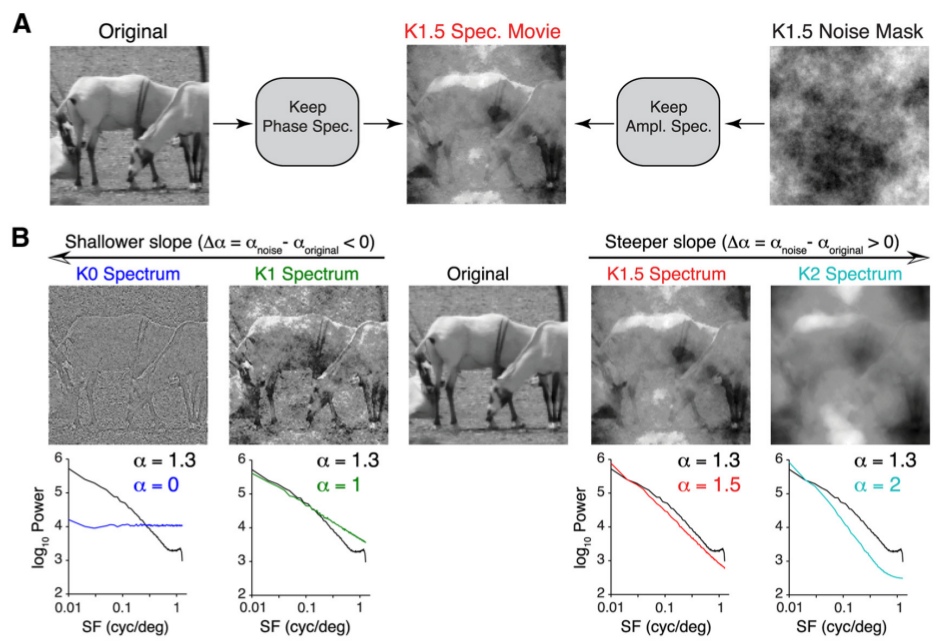
\includegraphics[width=.8\linewidth]{img/noise.png}
    \caption{Process of making noise movies}
    \label{img:noise}
\end{figure}
% subsectio\n setup (end)
\subsection{Data} % (fold)
\label{sub:data}
MATLAB datafile AmpMov.mat contains the following fields.\\
Experiments are done various days, the data corresponding to each day are in each folder.\\
Subscript \_nat corresponds to responses to video stimuli for original natural scenes video. similarly subscripts \_K0, \_K\_1, \_K1\_5, \_K\_2 denote responses to manipulated natural scenes video stimuli.\\
There are 6 different video stimuli. Each of them have 5 trials of experiment. Each trial is presenting a video sandwiched in gray non-stimuli. In each of this trial, every neuron sampled produced a time-series of 200 samples as response.
\begin{center}
    \begin{tabular}{|l|l|}
        \hline
        Field                                 & Description \\
        \hline
        Sorted.SpikeRate                  & No doc \\
        Blank                             & Dimension 47 x 16800 \\
        NumNeurons                        & Number of neurons sampled \\
        NumMovies                         & Number of movies used as stimulus \\
        M\_nat                            & Dimension 5 x 47 x 1200 \\
        MT\_nat                           & Dimension 5 x 47 x 200 x 6 \\
        MTA\_nat                          & Dimension 5 x 47 x 200 \\
        MTNA\_nat                         & Dimension 5 x 47 x 1200 \\
        \hline    
    \end{tabular}
\end{center}

% subsection data (end)
% section experiment (end)

\section{Study of Reliability} % (fold)
\label{sec:study_of_reliability}
Here we analyze how reliable are the time series responses produced by a neuron to various trials of same stimuli. We would like to bring out a metric for quantifying reliability of a neuron. Also we analyze the orientation selectivity properties of these `reliable' neurons.\\
Plots of responses to various trials of same stimuli are given in Figure . The responses are not similar/ have less correlation. This demands further study to find what is conserved between trials.
\begin{figure}
    \centering
    \begin{subfigure}[b]{.48\textwidth}
        \centering
        \includegraphics[width=\linewidth]{\plt/visualMain_meanPlot_2016_02_05_13_03_29.pdf}
    \end{subfigure}
    ~
    \begin{subfigure}[b]{.48\textwidth}
        \centering
        \includegraphics[width=\linewidth]{\plt/visualMain_meanPlot_2016_02_05_13_03_46.pdf}
    \end{subfigure}
    \caption{Responses of two neurons to various trials of same stimuli.}
    \label{img:responses}
\end{figure}
To quantify a neurons reliability,  we use following reliability measure. Response reliability to movie A ($R_A$ ) is calculated using the
following equation:
$$R_A = \frac{2}{T^2 - T}\sum_{i=1}^T \sum_{j=i+1}^T \rho(f_{i, A}, f_{j, A})$$
where $f_{i, A}$ is the response of neuron to $i^{th}$ trial of movie A and $\rho$ is the Pearson correlation.\\

\begin{figure}
    \centering
    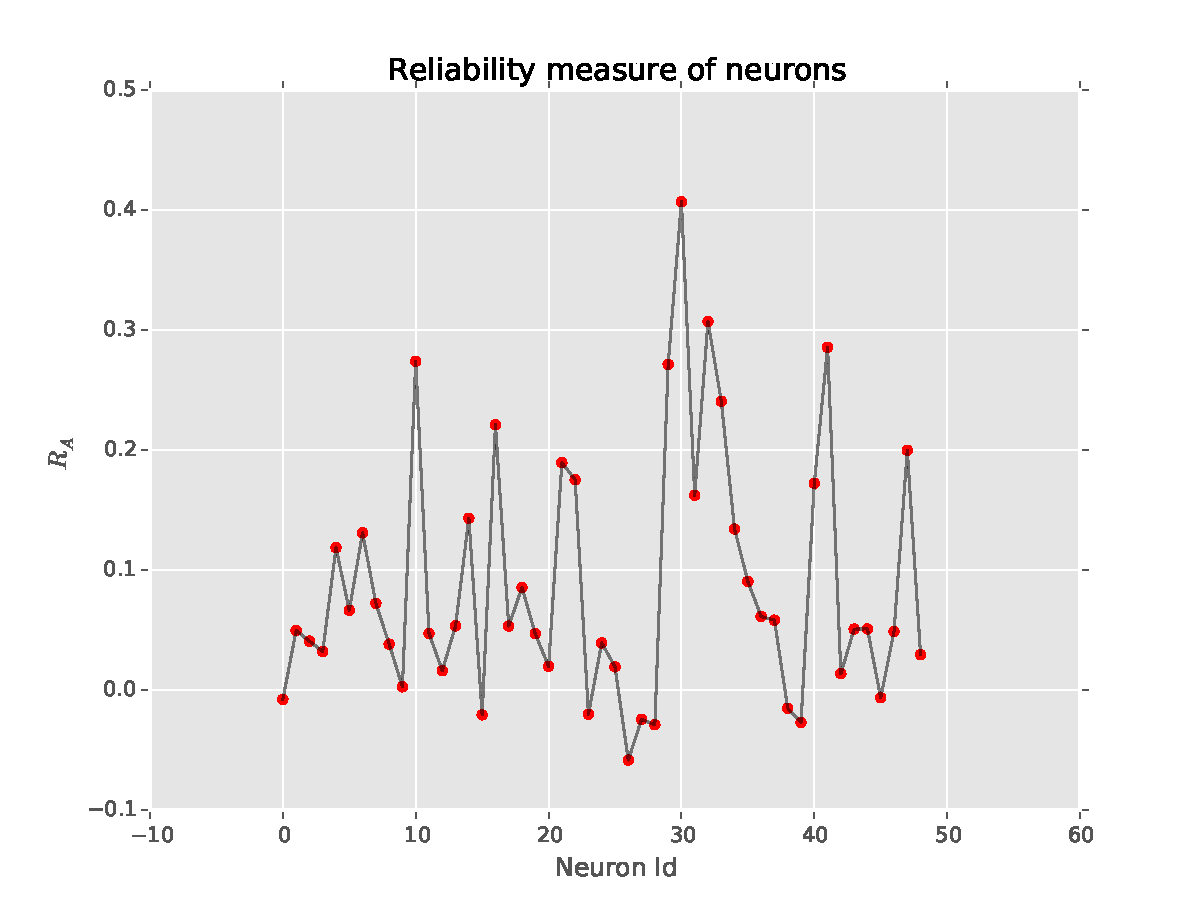
\includegraphics[width=.5\linewidth]{\plt/reliabMain_raPlot_2016_02_05_13_25_56.pdf}
    \caption{Reliability measure $R_A$ for different neurons}
    \label{img:ra}
\end{figure}
From figure~\ref{img:ra} is seen that the above measure is very low ($<0.4$) for most of the neurons. Which implies that the time series response is not the invariant structure we are looking for. 
% section study_of_reliability (end)

\section{Study of principal components} % (fold)
\label{sec:study_of_correlation}
It is known that there are three kinds of cells in V1 - simple, complex and orientation insensitive cells. Are there any correlation within these neurons? Is there redundancy in the code? We do an eigen analysis on the responses of all neurons in a mice to find how many uncorrelated dimensions are required to capture most of the variance.\\
Here we take number of neurons as feature dimension. The responses are averages across trials to form each point in the feature space. Every such time series responses were stacked to form the rows. Then PCA is done on the data to find number of components to variance explained ratio. Figure~\ref{img:pca} shows the result for a mouse towards a sinusoidal grating stimuli.
\begin{figure}
    \centering

\end{figure}\\
It is evident that original basis contain correlation/have features that doesn't contribute to variance in data. We project the original data to a smaller Eigen basis which capture most of the variance. Two studies are possible with this:
\begin{enumerate}
    \item Recreate the initial data from subset of principal components- Check how many principal components it takes for reasonable reconstruction.
    \item Do Further analysis like Orientation selectivity analysis with these data in Eigen space.
\end{enumerate}
\subsection{Reconstruction} % (fold)
\label{sub:reconstruction}
We study the effect of number of principal components on information capacity on Figure \ref{img:reconstruction}. As we increase principal components, the error should decrease. And finally as the number components equal the original feature dimension, reconstruction error should vanish.
\begin{figure}
    \centering
    \begin{subfigure}[b]{.48\textwidth}
        \centering
        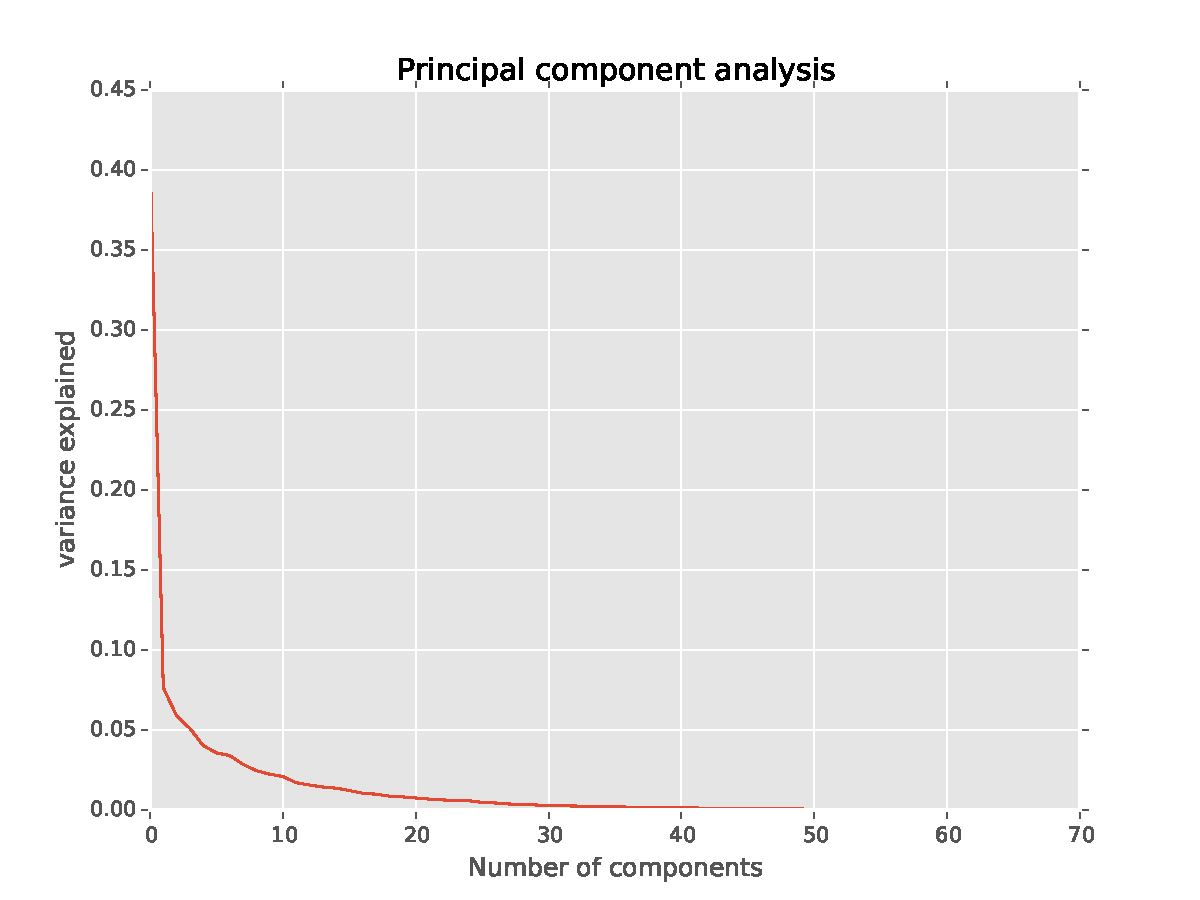
\includegraphics[width=\linewidth]{\plt/subsetbMain_pcaPlot_2016_02_05_15_41_05.pdf}
        \caption{Variance captured by components}
        \label{img:pca}
    \end{subfigure}
    ~
    \begin{subfigure}[b]{.48\textwidth}
        \centering
        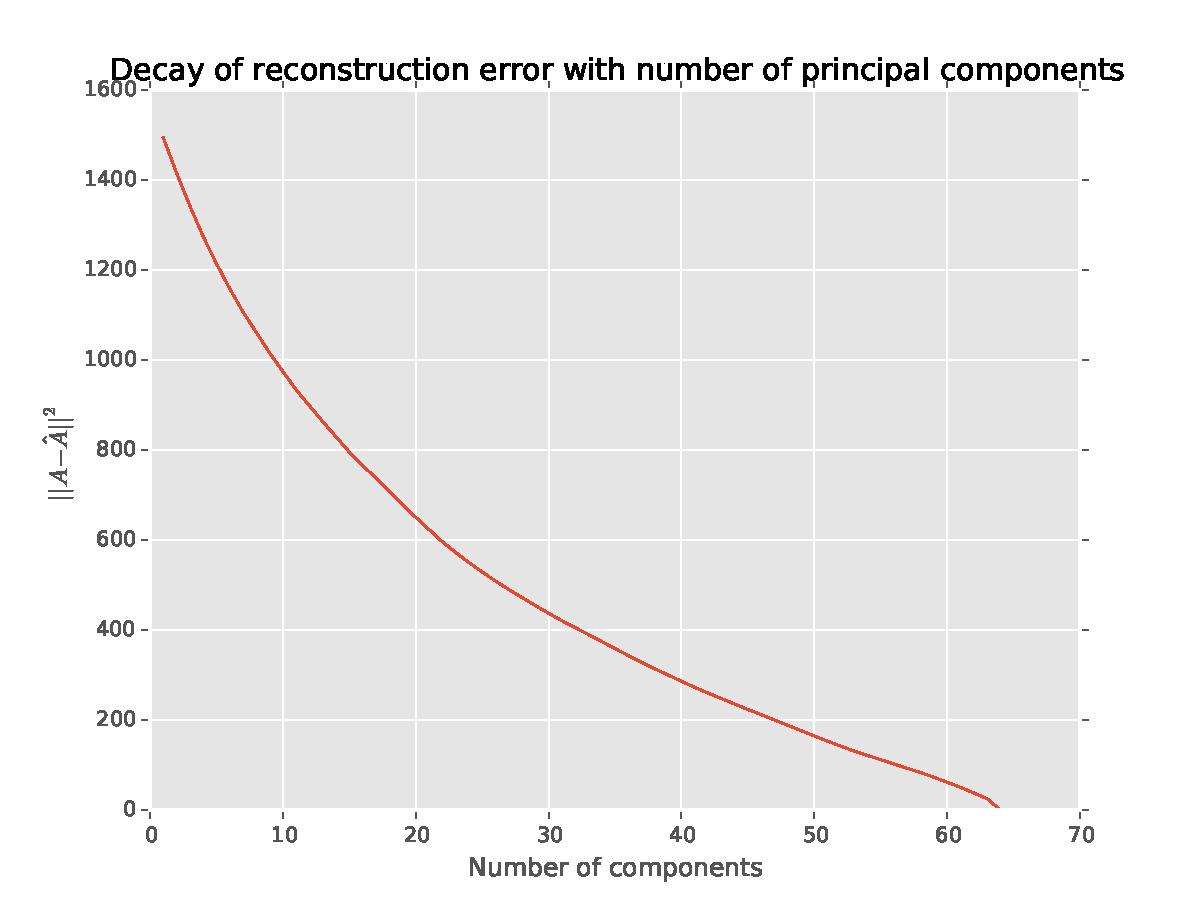
\includegraphics[width=\linewidth]{\plt/subsetbMain_errPlot_2016_02_12_12_42_39.pdf}
        \caption{Decay of reconstruction error}
        \label{img:reconstruction}
    \end{subfigure}
    \caption{Principal Components Analysis.}
\end{figure}
% subsection reconstruction (end)
\subsection{OSI analysis on data in Eigen space} % (fold)
\label{sub:osi_analysis_on_data_in_eigen_space}
The transformed data - the data with uncorrelated basis is studied here as if they are produced by neurons in V1. We call it `Eigen neurons' here. Will we be able to find an uncorrelated set of neurons?\\
To know if such a study makes sense, we plot average response with orientation. If it forms a double Gaussian,  we can go further. Figure shows response to orientation and clearly it does not form double Gaussian. Thus, further study in this regard is not proceeded.
% subsection osi_analysis_on_data_in_eigen_space (end)
% section study_of_correlation (end)



\section{Searching for subsequences} % (fold)
\label{sec:searching_for_motifs}
If the whole sequences are not reliable, could there be subsequences that are reliable? These motifs can repeat within response of the same neuron, or in a different trial, or in a different neuron. In this section, we search for such segments using ACVF.\\
For the scope of this section, `template' neuron is the neuron from which we take a subsequence to check for its other occurrences in the response of a `target' neuron.
When template and target is same neuron, we study repeated occurrences of a subsequence in a neuron's response.\\
Here, the search space is exponential in length of response. So before arriving at a method to reduce the search space, we analyze ACF with manually set template subsequence. Trial averaged responses of two neurons- template and target are taken, then a subset of former is extracted by frame ending and frame width. This is compared with target sequence as a function of lag. The results for this study with a subsequence starting from beginning of signal and of various widths are in Figure~\ref{img:acf1} for same neuron and figure~\ref{img:acf2} for different neurons.

\begin{figure}
    \centering
    \begin{subfigure}[b]{.48\textwidth}
        \centering
        \includegraphics[width=\linewidth]{\plt/acfMain_acfPlot_2016_02_05_16_49_00.pdf}
    \end{subfigure}
    ~
    \begin{subfigure}[b]{.48\textwidth}
        \centering
        \includegraphics[width=\linewidth]{\plt/acfMain_acfPlot_2016_02_05_16_49_09.pdf}
    \end{subfigure}
    \\
    \begin{subfigure}[b]{.48\textwidth}
        \centering
        \includegraphics[width=\linewidth]{\plt/acfMain_acfPlot_2016_02_05_16_52_16.pdf}
    \end{subfigure}
    ~
    \begin{subfigure}[b]{.48\textwidth}
        \centering
        \includegraphics[width=\linewidth]{\plt/acfMain_acfPlot_2016_02_05_16_49_27.pdf}
    \end{subfigure}
    \caption{ACF plots for template and target neurons as same.}
    \label{img:acf1}
\end{figure}

\begin{figure}
    \centering
    \begin{subfigure}[b]{.48\textwidth}
        \centering
        \includegraphics[width=\linewidth]{\plt/acfMain_acfPlot_2016_02_05_16_45_21.pdf}
    \end{subfigure}
    ~
    \begin{subfigure}[b]{.48\textwidth}
        \centering
        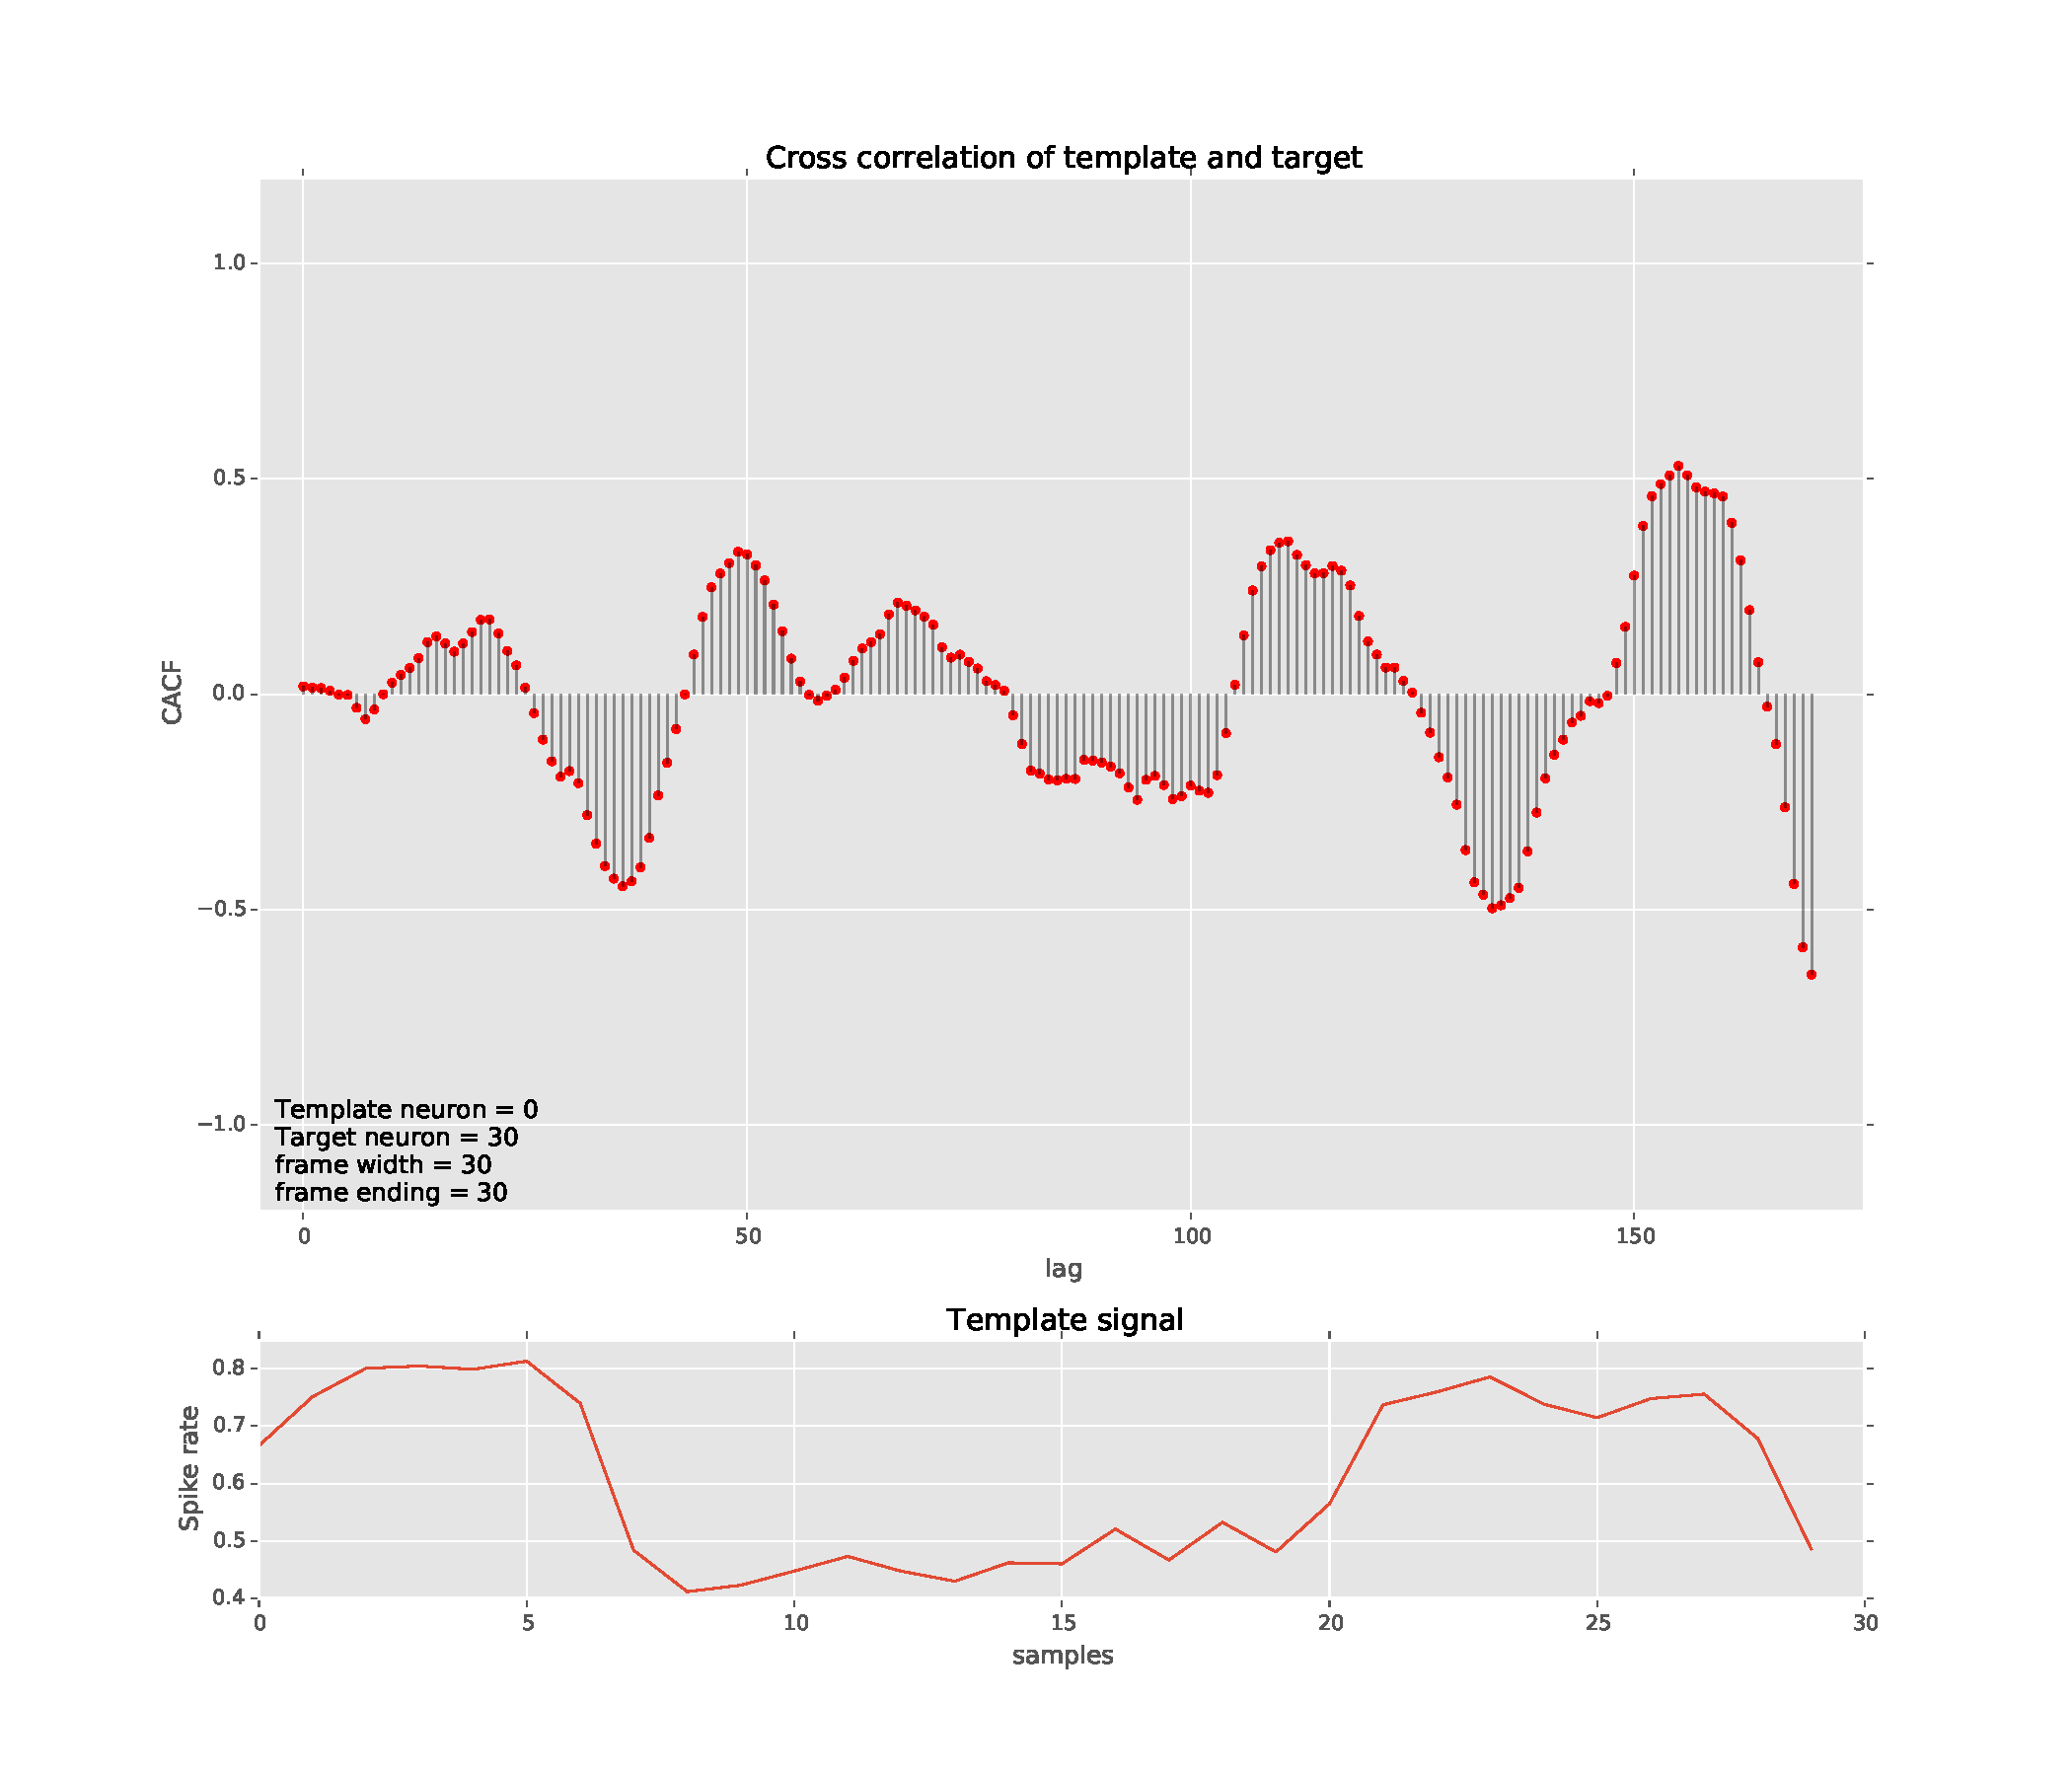
\includegraphics[width=\linewidth]{\plt/acfMain_acfPlot_2016_02_05_16_45_37.pdf}
    \end{subfigure}
    \\
    \begin{subfigure}[b]{.48\textwidth}
        \centering
        \includegraphics[width=\linewidth]{\plt/acfMain_acfPlot_2016_02_05_16_45_48.pdf}
    \end{subfigure}
    ~
    \begin{subfigure}[b]{.48\textwidth}
        \centering
        \includegraphics[width=\linewidth]{\plt/acfMain_acfPlot_2016_02_05_16_45_57.pdf}
    \end{subfigure}
    \caption{ACF plots for template and target neurons as different .}
    \label{img:acf2}
\end{figure}

\FloatBarrier
\subsection{ACF Gram} % (fold)
\label{sub:acf_gram}
In the previous study, we fixed the beginning of the frame in template and changed the width of frame. Here we will slide the frame also to create a temporal dimension too. Heatmaps of the ACF gram - a time vs lag vs ACVF plot are given in figure~\ref{img:acfgram1} for same neuron and figure~\ref{img:acfgram2} for different neurons.\\
Images show results for for different manually fixed window widths. The following inferences can be taken:
\begin{itemize}
    \item For small window length ($\approx$ 15), the template is small. Such a small template does not satisfy as a motif. Also as the samples are less, estimate of sample correlation will be poor.
    \item For window lengths $\approx 30$ we see patterns. These shows that there are repeating subsequences in the response.
    \item The repeating patterns seem to be reappearing periodically in lag.
    \item For window widths $\approx 60$, there are two subsequences that match. Above this, Only match is for lag 0.
    \item There are common subsequences across different neurons.
\end{itemize}
\begin{figure}
    \centering
    \begin{subfigure}[b]{.48\textwidth}
        \centering
        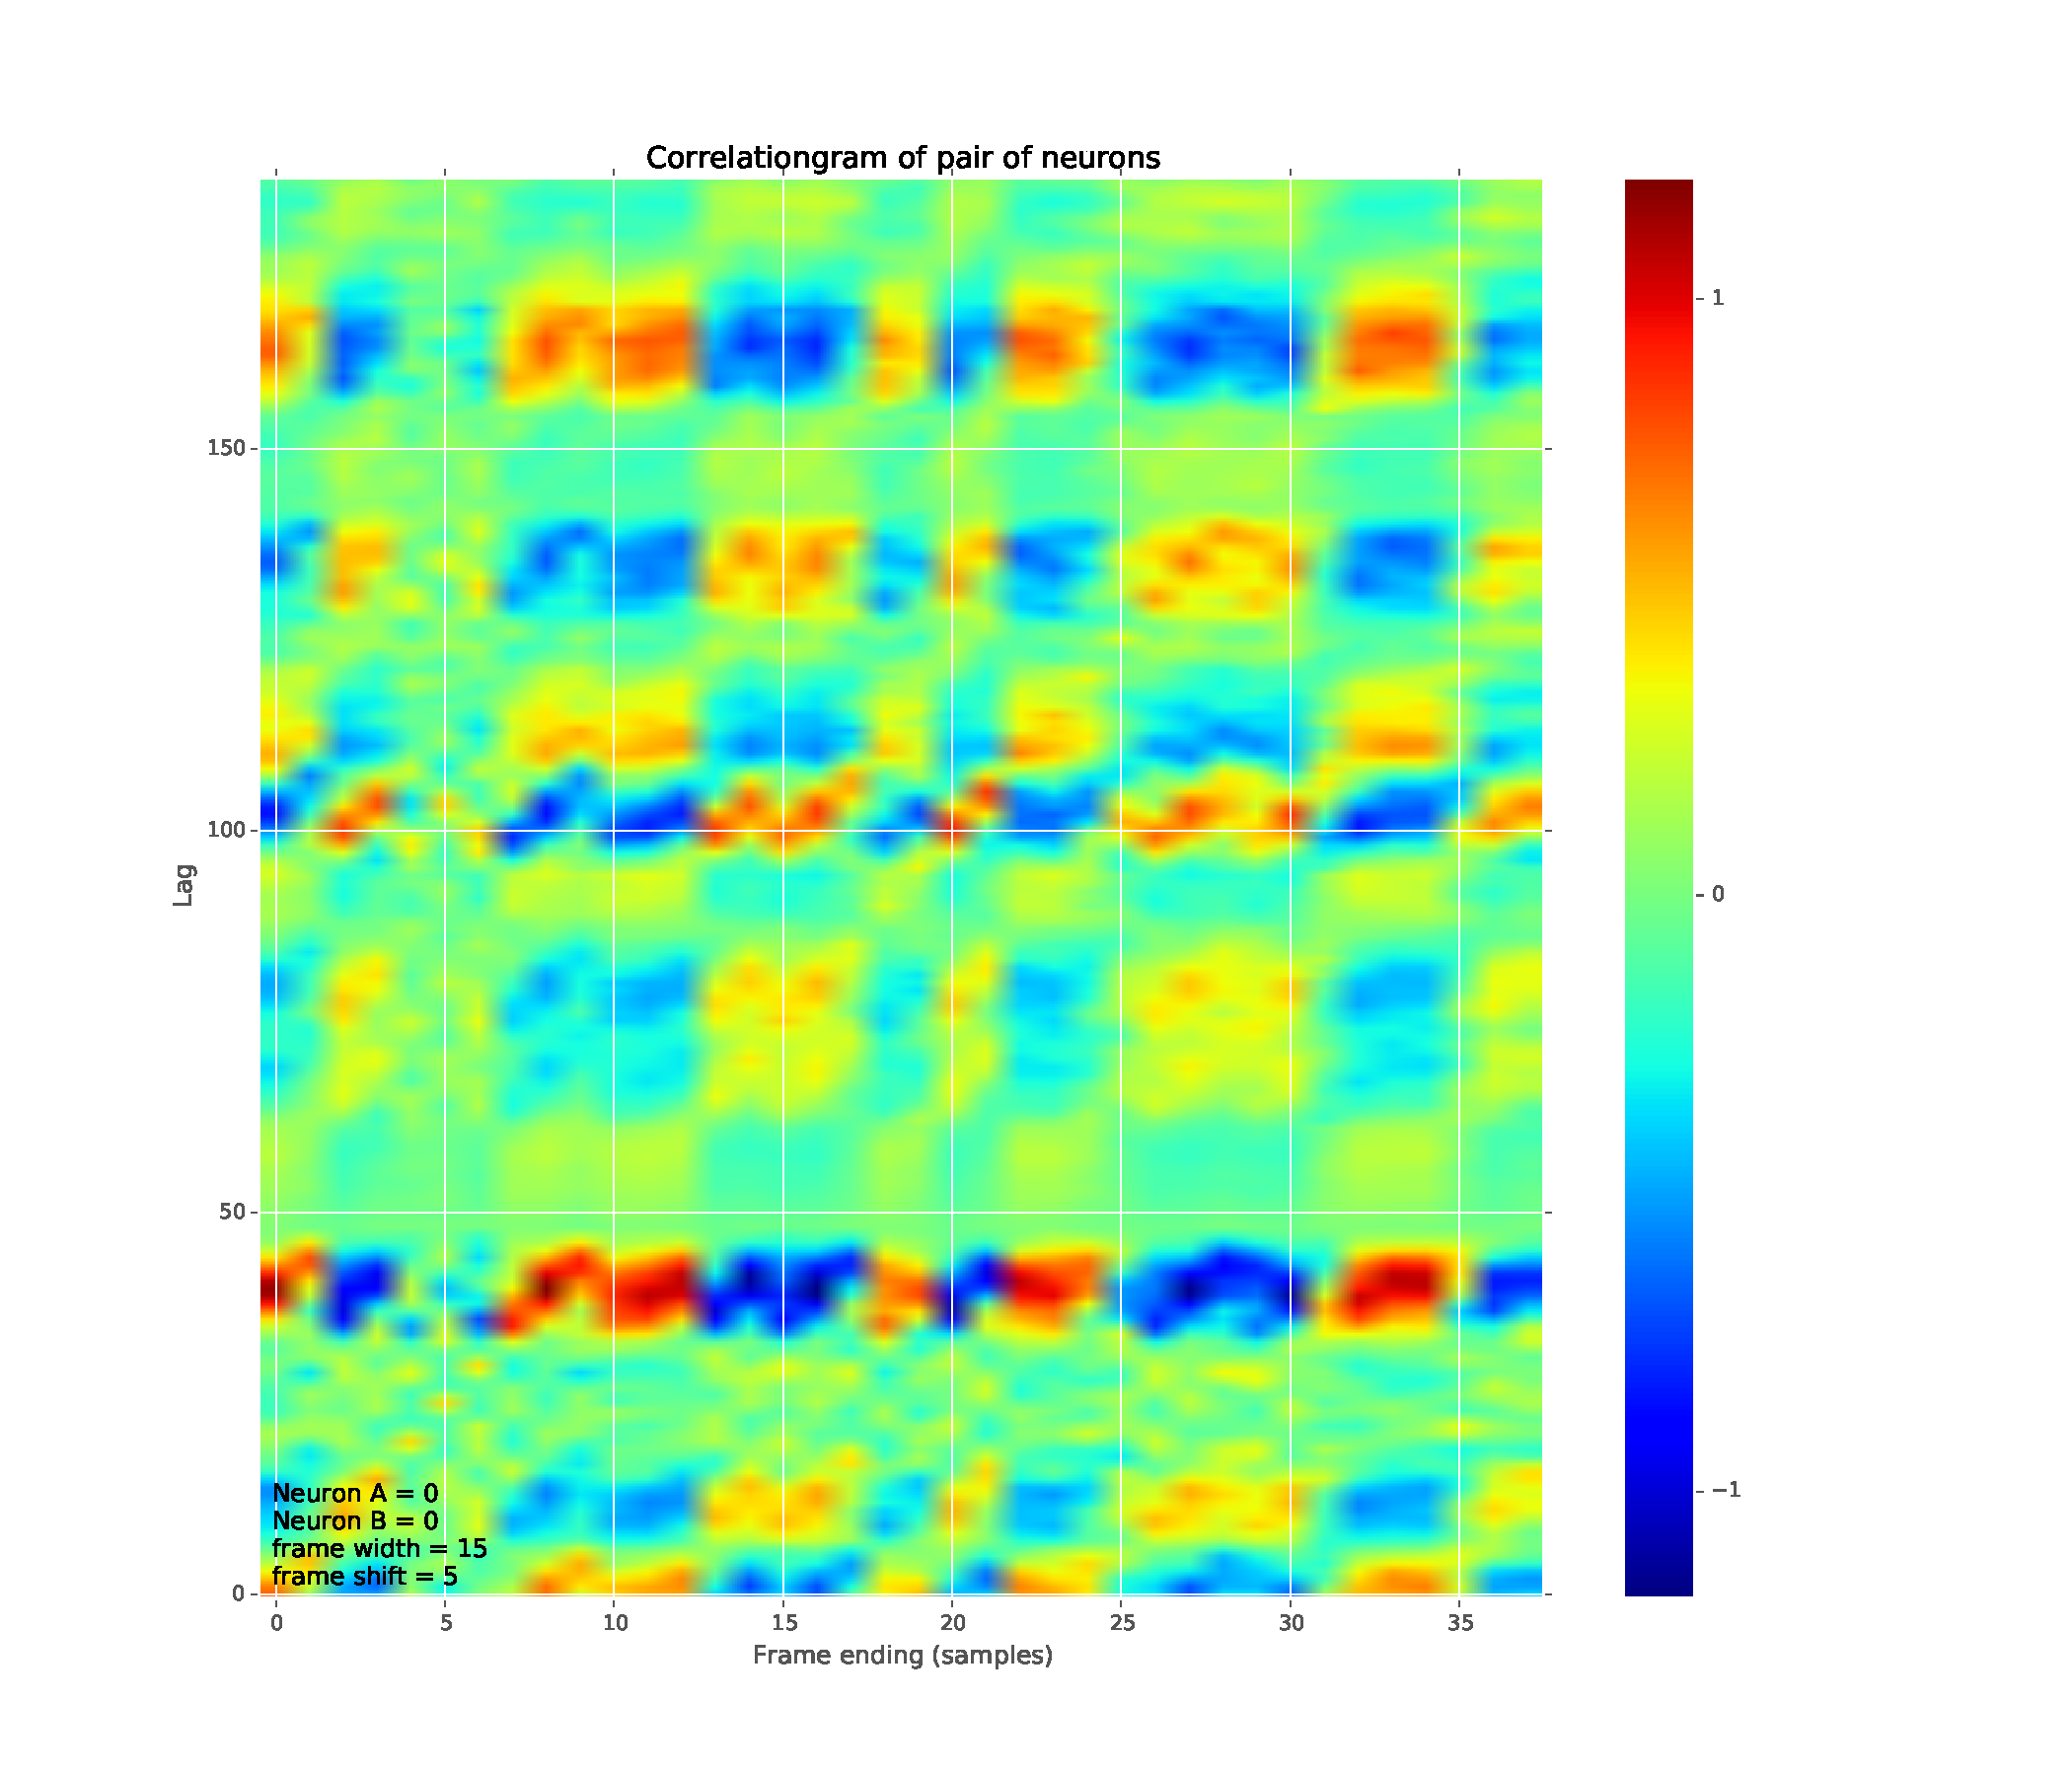
\includegraphics[width=\linewidth]{\plt/acfMain_corrGram_2016_02_05_16_49_00.pdf}
    \end{subfigure}
    ~
    \begin{subfigure}[b]{.48\textwidth}
        \centering
        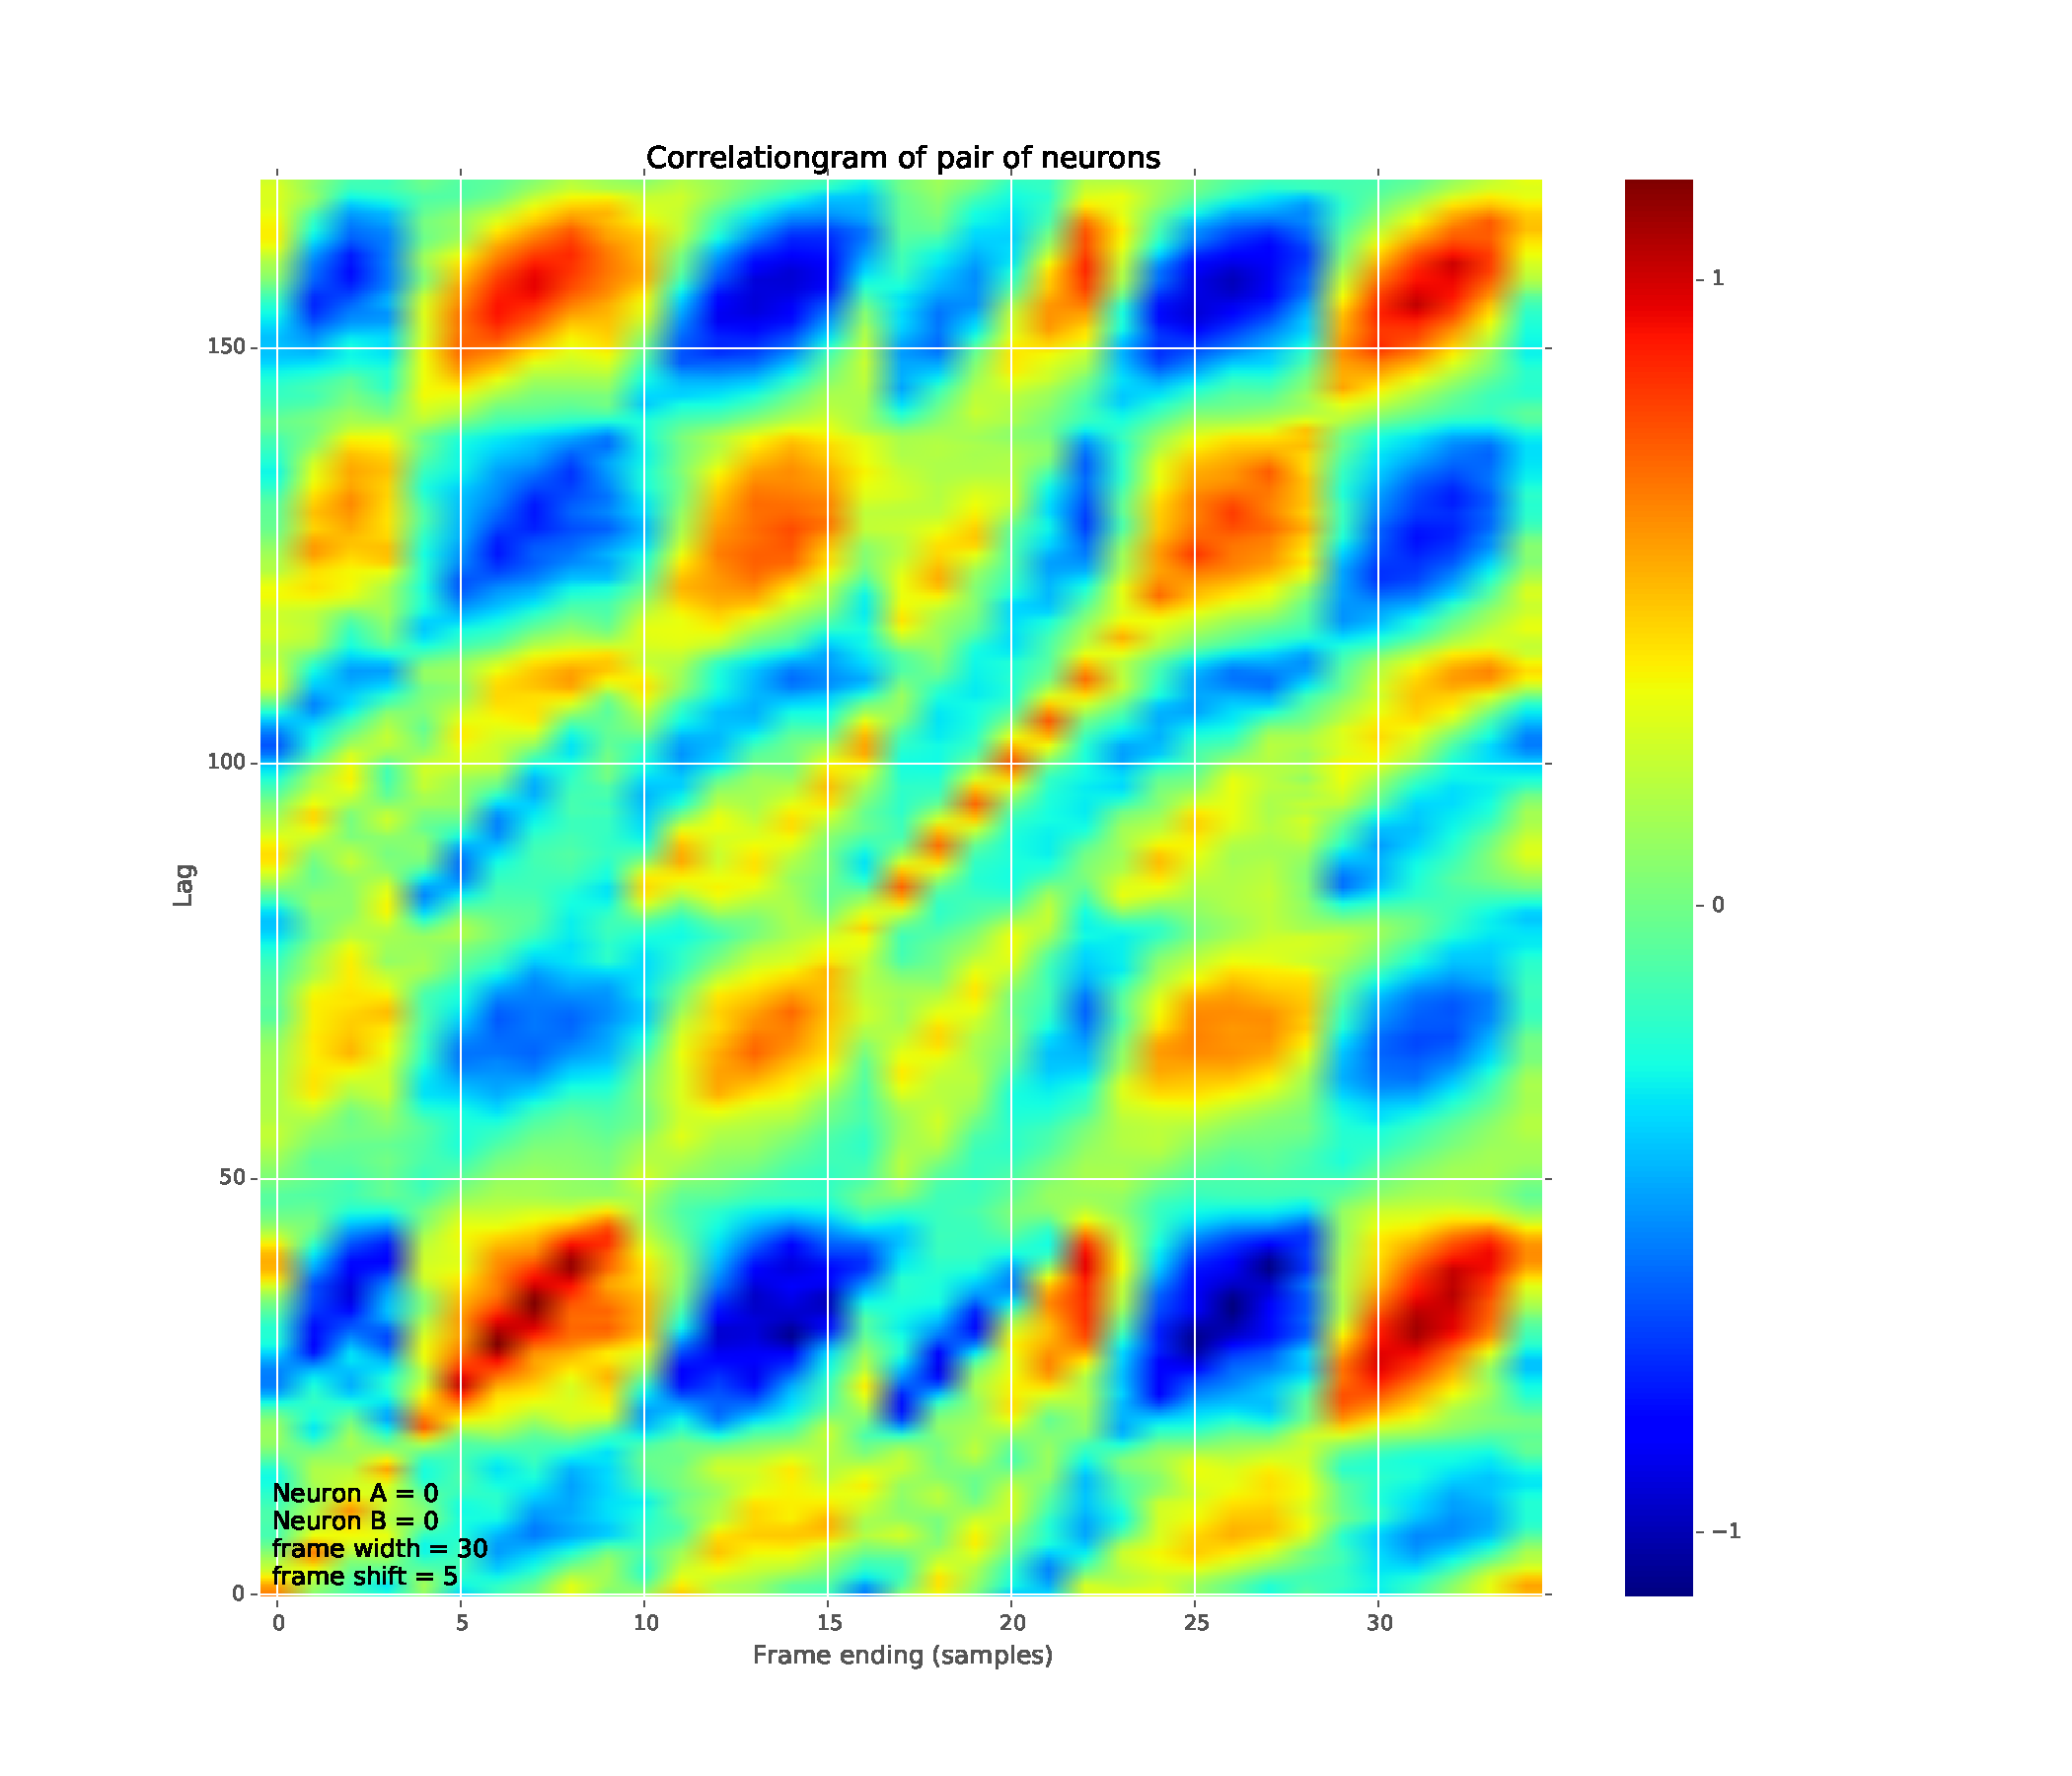
\includegraphics[width=\linewidth]{\plt/acfMain_corrGram_2016_02_05_16_49_10.pdf}
    \end{subfigure}
    \\
    \begin{subfigure}[b]{.48\textwidth}
        \centering
        \includegraphics[width=\linewidth]{\plt/acfMain_corrGram_2016_02_05_16_52_17.pdf}
    \end{subfigure}
    ~
    \begin{subfigure}[b]{.48\textwidth}
        \centering
        \includegraphics[width=\linewidth]{\plt/acfMain_corrGram_2016_02_05_16_49_28.pdf}
    \end{subfigure}
    \caption{ACFgram for template and target neurons as same.}
    \label{img:acfgram1}
\end{figure}

\begin{figure}
    \centering
    \begin{subfigure}[b]{.48\textwidth}
        \centering
        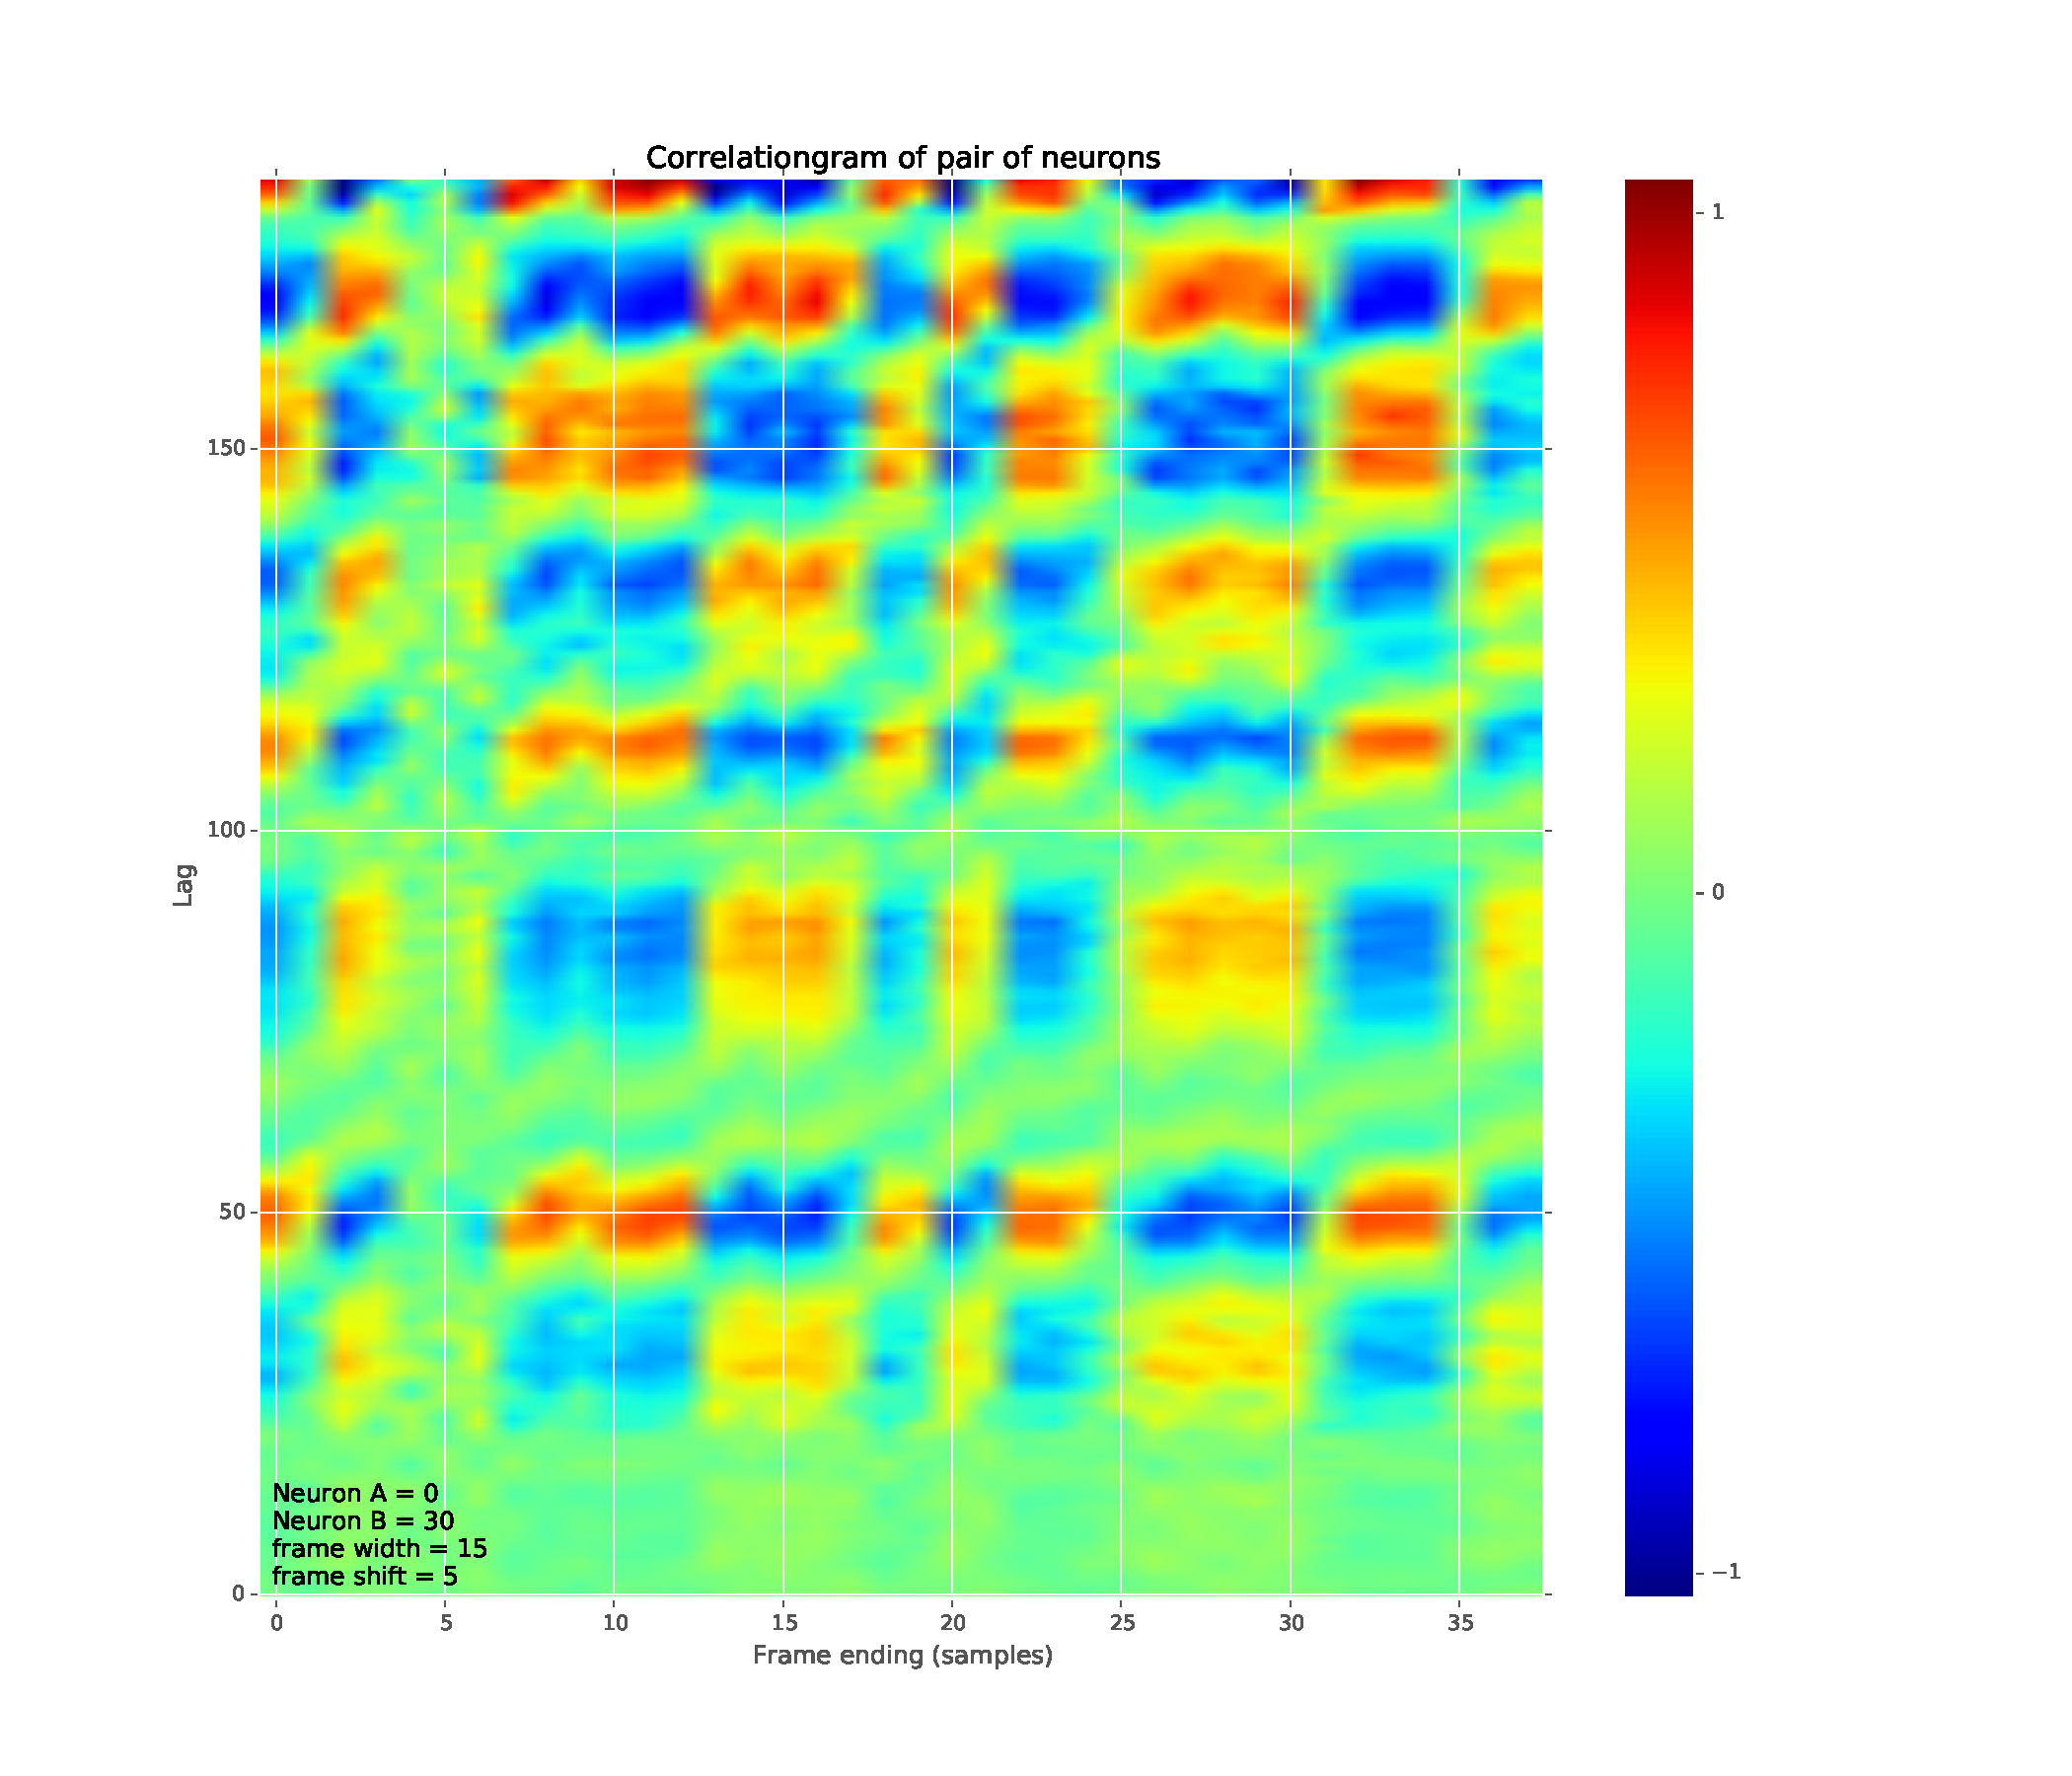
\includegraphics[width=\linewidth]{\plt/acfMain_corrGram_2016_02_05_16_45_22.pdf}
    \end{subfigure}
    ~
    \begin{subfigure}[b]{.48\textwidth}
        \centering
        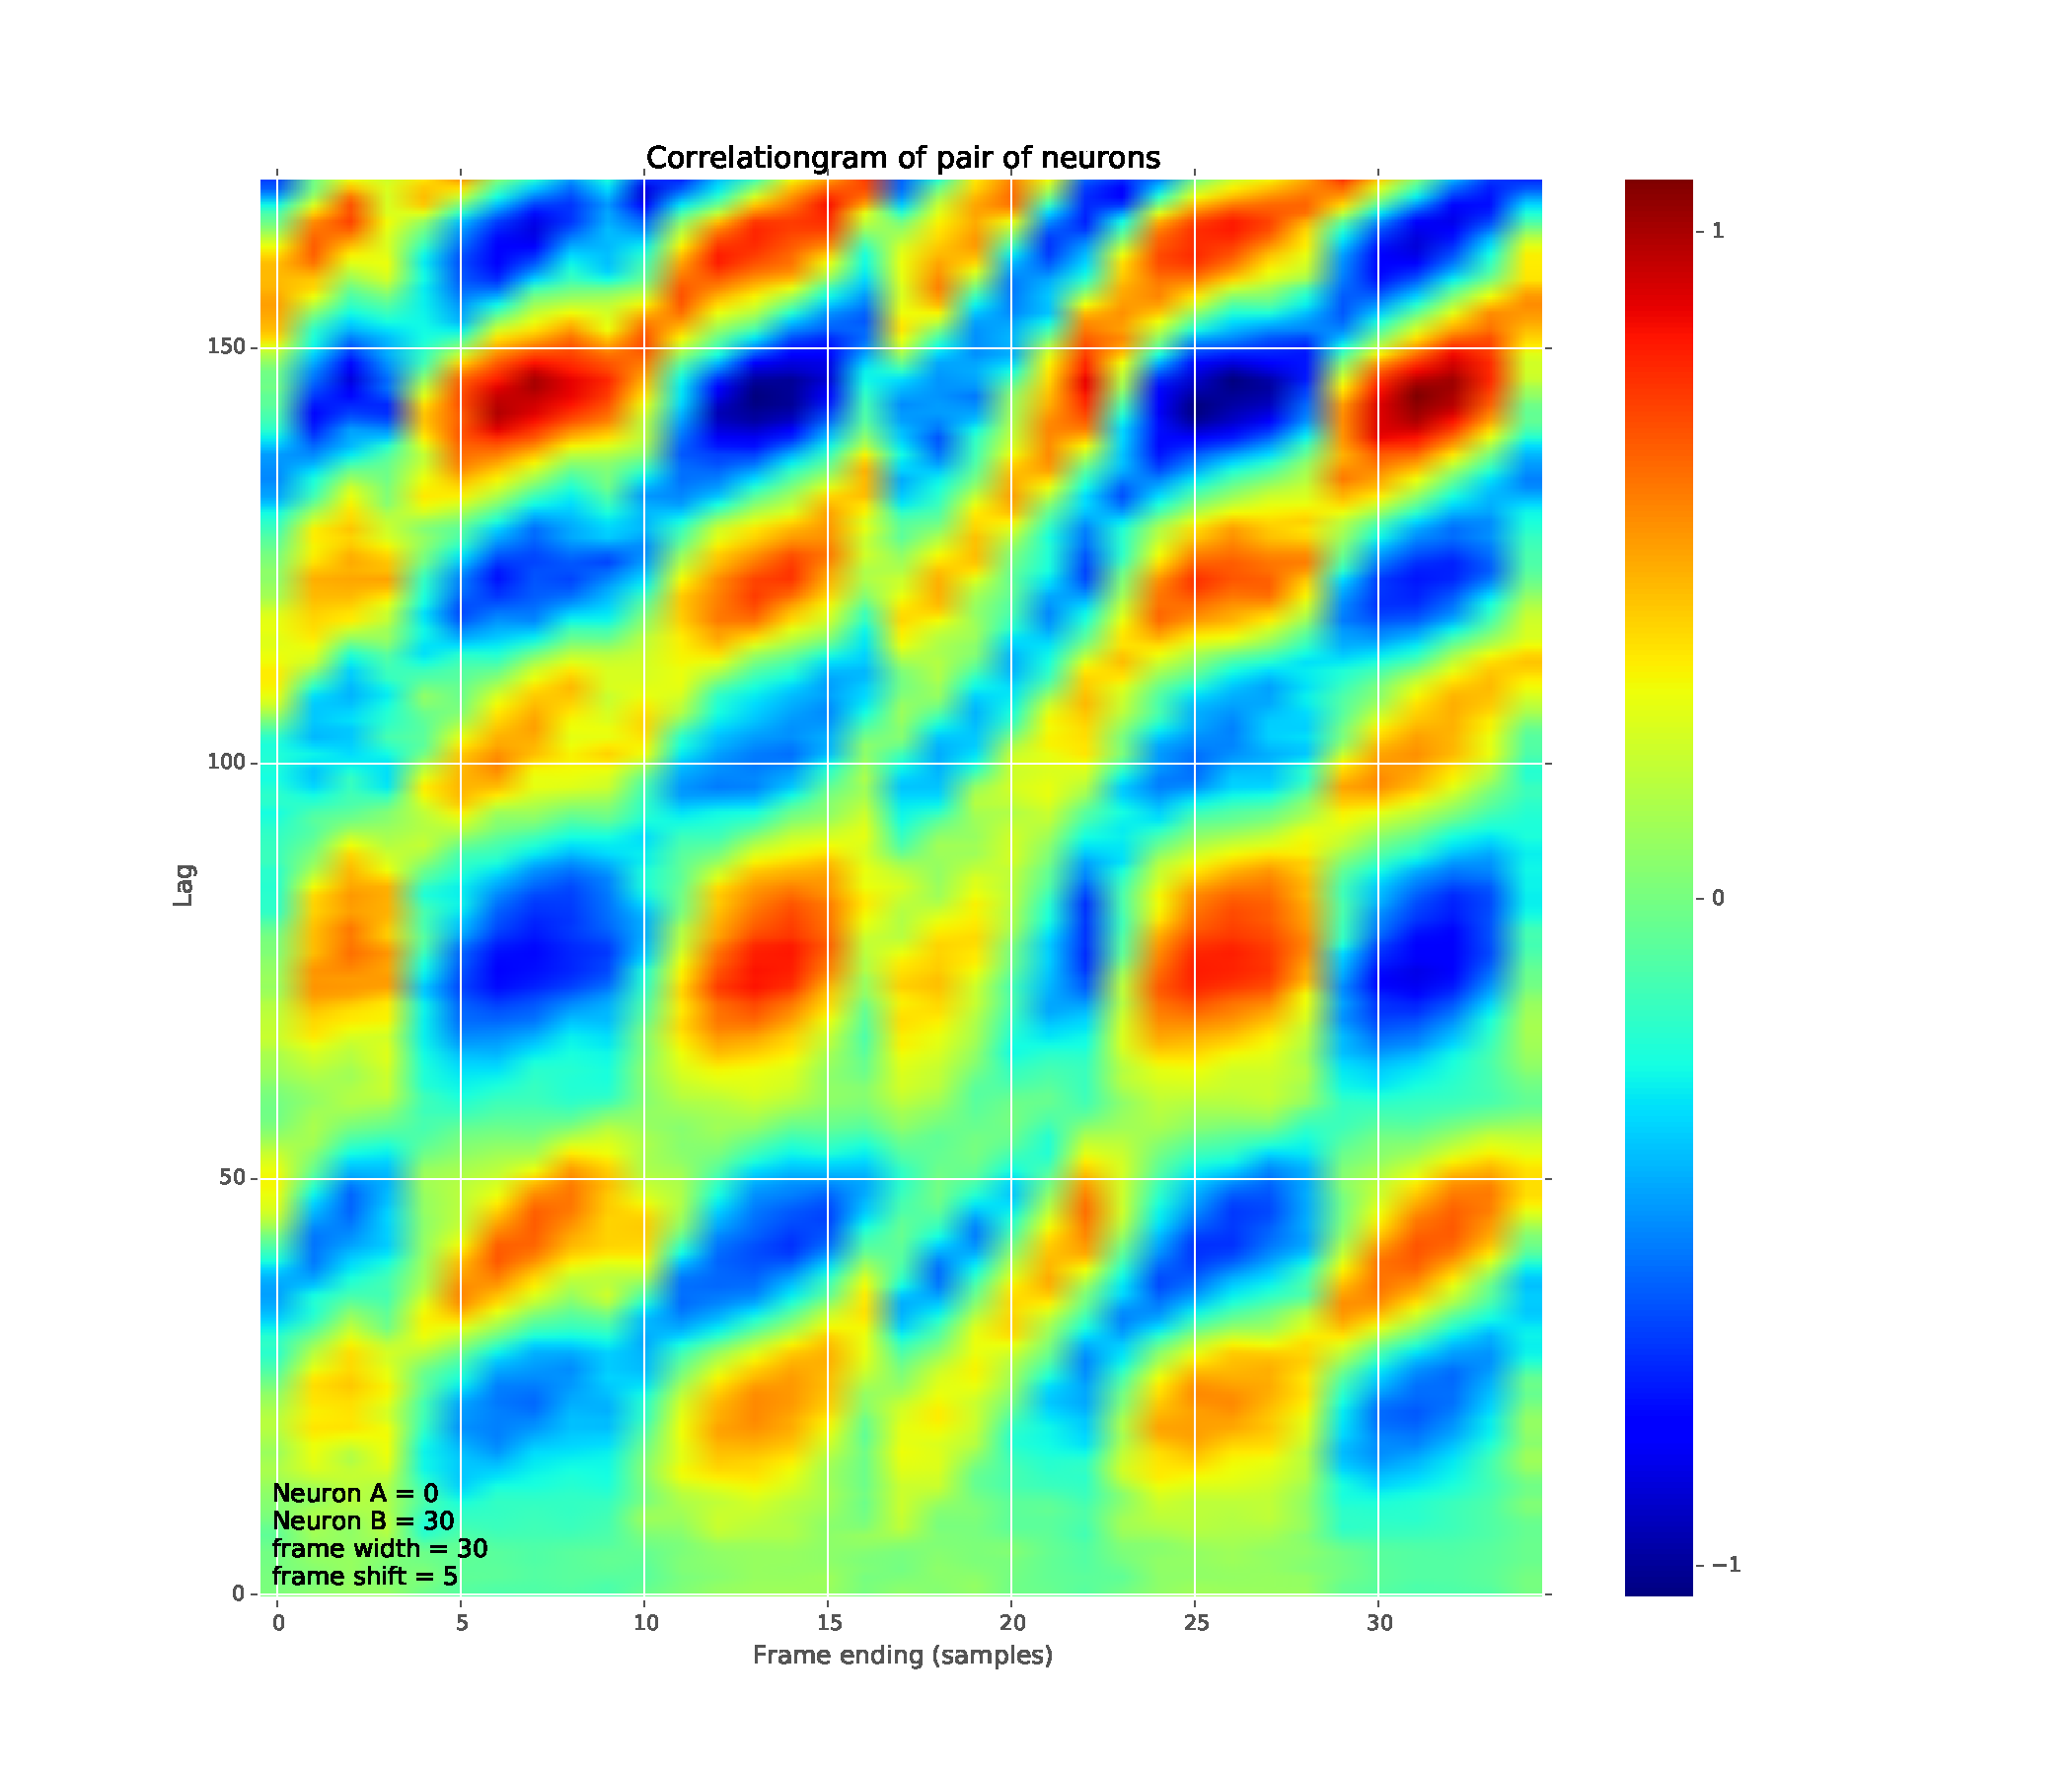
\includegraphics[width=\linewidth]{\plt/acfMain_corrGram_2016_02_05_16_45_38.pdf}
    \end{subfigure}
    \\
    \begin{subfigure}[b]{.48\textwidth}
        \centering
        \includegraphics[width=\linewidth]{\plt/acfMain_corrGram_2016_02_05_16_45_48.pdf}
    \end{subfigure}
    ~
    \begin{subfigure}[b]{.48\textwidth}
        \centering
        \includegraphics[width=\linewidth]{\plt/acfMain_corrGram_2016_02_05_16_45_57.pdf}
    \end{subfigure}
    \caption{ACFgram for template and target neurons as different .}
    \label{img:acfgram2}
\end{figure}
% subsection acf_gram (end)

\subsection{Longest common subsequences} % (fold)
\label{sub:longest_common_subsequences}
In previous study, we fixed the window widths and saw that there are in fact repeating patterns. Here we try to find set of common subsequences in neurons. Also, till now we used Pearson correlation to compare two signals. We look into other ways of comparing two responses too.
\subsubsection{Longest common segment set for neuron responses} % (fold)
\label{ssub:longest_common_segment_set_for_neuron_responses}
Here we compare responses of two neurons- template and target neurons. Both signals are time series signals obtained by averaging responses to each trial of the same stimuli. Subsequence matching needs to be performed
between these two signals. The number of similar portions could be more than one and spread across the entire signal.\\
Let $\bm{X} = < x_1, x_2,\hdots, x_n ; x_i \in R >$ be template signal and $\bm{Y} = <y_1, y_2, \hdots, y_m ; y_m \in R>$ be the target signal. Now similarity between two points has to be defined. Following options of similarity measures are considered.
\begin{enumerate}
    \item Euclidean distance\\
    $$sim(x_i, y_j) =  (x_i - y_j)^2$$
    \item Cubic\\
    $$sim(x_i, y_j) =  1 - (x_i - y_j)^3$$
\end{enumerate}
Classic problem of finding LCSS is as follows:
$$
LCS\left(X_{i},Y_{j}\right) =
\begin{cases}
  \emptyset
& \mbox{ if }\ i = 0 \mbox{ or }  j = 0 \\
  \textrm{  } LCS\left(X_{i-1},Y_{j-1}\right) \frown x_{i}
& \mbox{ if } sim(x_i , y_j) > \tau_{sim} \\
  \mbox{longest}\left(LCS\left(X_{i},Y_{j-1}\right),LCS\left(X_{i-1},Y_{j}\right)\right)
& \mbox{ if } sim(x_i , y_j) < \tau_{sim} \\
\end{cases}
$$
We can solve this problem by Dynamic Programming.
\newpage
\section{**Future work}
\begin{enumerate}
    \item LCSS on neural response\\
    Perform LCSS to find common subsequences in responses of two neurons. For this we can use different similarity functions.\\
    On performing LCSS on two neurons, the scores matrix generated is in Figure
    \begin{figure}
        \centering
        \includegraphics[width=.7\linewidth]{\plt/lcssMain_scoremat_2016_02_23_16_52_00}
        \caption{Score matrix after LCSS on two neuron responses}
    \end{figure}
    \item RLCS\\
    Perform RLCS to match sequences.
    \item Multi dimensional extension\\
    Till now we were trying to find similarities between two neurons. We need to analyze neurons as a population.\\
    Extend methods above for multi dimension/ population of neurons.
\end{enumerate}
% subsubsection longest_common_segment_set_for_neuron_responses (end)
% subsection longest_common_subsequences (end)
% section searching_for_motifs (end)
% ============================== Content ends here
\end{document}